\subsection{Vector-Valued Functions}

\purple{\From Section 1.8 of \VCT.}

\BEN

%% ~~~~~~~~~~~~~~~~~~~~~~~~~~~~~~~~~~~~~~~~~~~~~~~~~~~~~~~~~
%\item
%% QUESTION 
%For $A$ and \textbf{b} below, solve the linear system $A\mathbf{x} = \mathbf{b}$, if possible:
%\begin{align*}
% A = \BM
%  1 & 2 & 0 & 1 \\
%  3 & -1 & 1 & 2 \\
%  0 & 1 & 0 & 2 \\
%  4 & 0 & 3 & 1
% \EM, \ 
% \mathbf{b} = \BM 1 \\ 5 \\ 0 \\ 10 \EM.
%\end{align*}
% If it isn't possible to solve this system, explain why. 
%
%% ~~~~~~~~~~~~~~~~~~~~~~~~~~~~~~~~~~~~~~~~~~~~~~~~~~~~~~~~~
%\item
%% QUESTION 
%For the systems below,
%\begin{itemize}
%\item Compute the determinant of matrix $A$, if possible. If it is not possible to do so, explain why. 
%\item Solve the linear system $A\mathbf{x} = \mathbf{b}$, if possible. 
%\item State whether the system has no solution, infinitely many solutions, or a unique solution.
%\end{itemize}
%
%\begin{enumerate}
%\item \(
% A = \begin{bmatrix}
%  -3 &  1 & 2 &  4 \\
%   2 & -1 & 2 &  3 \\
%   1 &  0 & 4 & -2
% \end{bmatrix}, \ 
% \mathbf{b} = \begin{bmatrix} 1 \\ 1 \\ 1 \end{bmatrix}
%\)
%\item \( A = \begin{bmatrix}
% 1 & 2 & -1 \\
% 2 & 5 & 0 \\
% 4 & 9 & -2
%\end{bmatrix} , \ 
% \mathbf{b} =
%\begin{bmatrix} 1 \\ 2 \\ -1 \end{bmatrix} \)
%\end{enumerate}

% ~~~~~~~~~~~~~~~~~~~~~~~~~~~~~~~~~~~~~~~~~~~~~~~~~~~~~~~~~
\item 
% QUESTION
Find the values of $t$ and the points on the curve 
\begin{align*}
  \mathbf{r}(t) &= (1+t^2) \mathbf{i} + t\mathbf{j}, \quad t\in \R
\end{align*}
where
\begin{enumerate}
  \item $\mathbf{r}(t)$ and $\mathbf{r}'(t)$ are perpendicular,
  \item $\mathbf{r}(t)$ and $\mathbf{r}'(t)$ have the same direction, and
  \item $\mathbf{r}(t)$ and $\mathbf{r}'(t)$ have opposite directions.   
\end{enumerate}
%
%% ~~~~~~~~~~~~~~~~~~~~~~~~~~~~~~~~~~~~~~~~~~~~~~~~~~~~~~~~~
%\item 
%% QUESTION 4
%%GPS: MMCA2b
%
%Consider the system of simultaneous linear equations
%\begin{align*}
%  x + 2y -  z &= 2 \\
% 2x + ay - 2z &= b \\
% 3x + 2y      &= 1
%\end{align*}
%where $x, y, z$ are unknown.
%
%\begin{enumerate}
%\item Find all values of $a$ and $b$ such that the above system has
%\begin{enumerate}
%\item \label{q:one_solution} exactly one solution;
%\item no solutions;
%\item \label{q:many_solutions} infinitely many solutions.
%\end{enumerate}
%\item For those values of $a$ and $b$ from~\ref{q:one_solution}, what is the
%unique solution?
%\item For those values of $a$ and $b$ from~\ref{q:many_solutions},
% parameterize the set of all solutions.
%\end{enumerate}
%
%% ~~~~~~~~~~~~~~~~~~~~~~~~~~~~~~~~~~~~~~~~~~~~~~~~~~~~~~~~~
%
\item \textbf{Application to Mechanics}\\
%For $t\in\R$, the real valued functions
%\begin{align*}
%y(t)=2+5t, \quad y(t) = \sin(4t) , \quad y(t)=e^{6t}
%\end{align*}
%are referred to as \textbf{scalar functions}, because in each case, they assign a real number $y$, to another real number $t$. However, functions such as
%\begin{align*}
%\mathbf{v}(t)=\mathbf{r}_0+t\mathbf{r}, \quad \mathbf{v}(t) = \sin(4t)\mathbf{a} , \quad \mathbf{v}(t)=e^{6t}\mathbf{b}
%\end{align*}
%assign a vector to real numbers, and are referred to as \textbf{vector functions}. They could be used, for example if the position of a particle is specified by the vector $\mathbf{r}\in \R^3$, and that the particle is moving, so that \textbf{r} is a function of time: \textbf{r}=\textbf{r}$(t)$. 
%
%Many of the properties of vector functions are intuitive. For example, the derivative of a vector function, defined as
%\begin{align*}
%\lim_{h\rightarrow0} \frac{\mathbf{r}(t+h) - \mathbf{r}(t)}{h}
%\end{align*}
%describes the rate of change of $\mathbf{r}$ at $t$ (provided that the limit exists). If the vector \textbf{r} represents the position of a particle at time $t$, then, naturally, $\mathbf{r}'(t)$ represents its velocity at time $t$, and $\mathbf{r}''(t)$ represents its acceleration at time $t$. Moreover, we can compute the derivative of a vector by simply taking the derivative of each of its components separately. For example, if $\mathbf{v}(t) = 5t \mathbf{i} + \cos(t)\mathbf{j} - \mathbf{k}$, then $\mathbf{v}'(t) = 5 \mathbf{i} - \sin(t)\mathbf{j} - 0 \mathbf{k}$, or 
%\begin{align*}
% \frac{d \mathbf{v}(t)}{dt} = \mathbf{v}'(t) &= \BM 5 \\ -\sin(t) \\ 0 \EM.
%\end{align*}
%Differentiation rules for scalar multiplication, cross and dot products can also be derived and resemble the product rule for scalar functions:
%\begin{align*}
%\frac{d}{dt} \big( C \mathbf{u}(t)\big) &=C \frac{d \mathbf{u}(t) }{dt}  , \quad C \text{ is a constant} \\
%\frac{d}{dt} \big( \mathbf{v}(t) \cdot \mathbf{u}(t)\big) &= \mathbf{v}(t) \cdot \frac{d \mathbf{u}(t) }{dt}  +  \frac{d \mathbf{v}(t)}{dt}  \cdot  \mathbf{u}(t) \\
%\frac{d}{dt} \big( \mathbf{v}(t) \times \mathbf{u}(t)\big) &= \mathbf{v}(t) \times \frac{d \mathbf{u}(t) }{dt}  +  \frac{d \mathbf{v}(t)}{dt}  \times  \mathbf{u}(t) 
%\end{align*}
%Other differentiation formulas that you may need throughout this course are provided in your textbook. \\\\
%\noindent\textbf{Questions}
Recall from a previous assignment that we defined torque as $\boldsymbol\tau = \mathbf{r} \times \MB{F}$. Now that we have introduced the concepts of vector-valued functions and their derivatives, let's consider the more general case when $\boldsymbol\tau$, $\MB{r}$, and $\MB{F}$ are all functions of time:
\begin{align*}
  \boldsymbol\tau(t) &= \mathbf{r}(t) \times \MB{F}(t).
\end{align*}
Moreover, using the relation $\MB{F}(t)=m\MB{a}(t)$ (Newton's second law), we can write our definition of torque as
\begin{align*}
  \boldsymbol\tau(t) &= \mathbf{r}(t) \times \MB{F}(t) \\
  &= \mathbf{r}(t) \times \big(m\MB{a}(t)\big) \\
  &= m\big( \mathbf{r}(t) \times \mathbf{r}''(t)\big).
\end{align*}
These alternate forms for the torque vector may be helpful in solving the following problems.
\begin{enumerate}
\item If the position of a particle with mass $m$ is given by the position vector $\mathbf{r}(t)$, then its angular momentum is a vector defined as $\mathbf{L}(t) = m\mathbf{r}(t)\times \mathbf{r}'(t)$. Show that $\mathbf{L}'(t) = \boldsymbol\tau(t)$.
\item Show that if the torque is a zero vector for all $t$, then the angular momentum of the particle is constant for all $t$. This is what is known as the \Emph{law of conservation of angular momentum}.
\end{enumerate}
%% ~~~~~~~~~~~~~~~~~~~~~~~~~~~~~~~~~~~~~~~~~~~~~~~~~~~~~~~~~
%% POLYNOMIAL INTERPOLATION 
%\item \textbf{Application to Polynomial Interpolation}
%
%In many areas of engineering, experimental data is collected that must be analyzed to extract parameters that tell us something about a physical process. Suppose we have measured a set of experimental data that are represented in the $xy$-plane. An \Emph{interpreting polynomial} for the measured data is a polynomial that passes through every measured point. We can use this polynomial, for example, to estimate values between the measured data points. \\
%
%Suppose for example that we have measured the data points (0,-6), (1,-2), (2,4), (3,10). To find an interpreting polynomial of order 2 for these data, we would try to find a polynomial of the form $p(x) = a_0+a_1x+a_2x^2$ that passes through all four measured points. In other words, we need to find the unknown constants $a_0, a_1, a_2$ that satisfy the equations
%\begin{align*}
%p(0) = a_0+a_1(0)+a_2(0)^2 &= -6 \\
%p(1) = a_0+a_1(1)+a_2(1)^2 &= -2 \\
%p(2) = a_0+a_1(2)+a_2(2)^2 &= 4  \\
%p(3) = a_0+a_1(3)+a_2(3)^2 &= 10 
%\end{align*}
%The above system has four equations and four unknowns. Upon solving this system, you should be able to determine that $a_0 = -6, a_1 = 4, a_2=0$.\\
%
%\textbf{Wind Tunnel Experiment}\\
%In a fictitious wind tunnel experiment, the following measurements were made. 
%\begin{center}
%  \begin{tabular}{ c c }
%    Velocity (m/s) & Force (N)  \\ \hline
%     0  & 0 \\
%    1 & 5.5 \\
%    2 & 20 \\
%    3 & 46.5 \\
%    4 & 88
%  \end{tabular}
%\end{center}
%
%The data represent the measured force due to air resistance, on an object suspended in the tunnel, measured at different air speed velocities.
%\begin{enumerate}
%\item Using the data above, derive a $5\times4$ system of equations, that when solved, find an interpreting polynomial of the form $p(x) = a_0+a_1x+a_2x^2+a_3x^3$. Write the system in the form $A\mathbf{x}=\mathbf{b}$.
%\item Solve your system to obtain $p(x) = a_0+a_1x+a_2x^2+a_3x^3$.
%\item As mentioned above, engineers sometimes use interpreting polynomials to estimate values in between measured data points. Using your polynomial, estimate the value of the force when the velocity is 1.5 m/s. 
%\item In practice, it can be difficult to determine what order of polynomial to use. Sometimes, polynomials of different orders must be used to decide which polynomial yields the most useful results. For the above data, explain what what would happen if we used a polynomial less than 3. It may help to see what happens if we use a 1$^{st}$ order polynomial. 
%\end{enumerate}
%\begin{figure}[h]
%  \vspace{-5pt}
%  \begin{center}
%    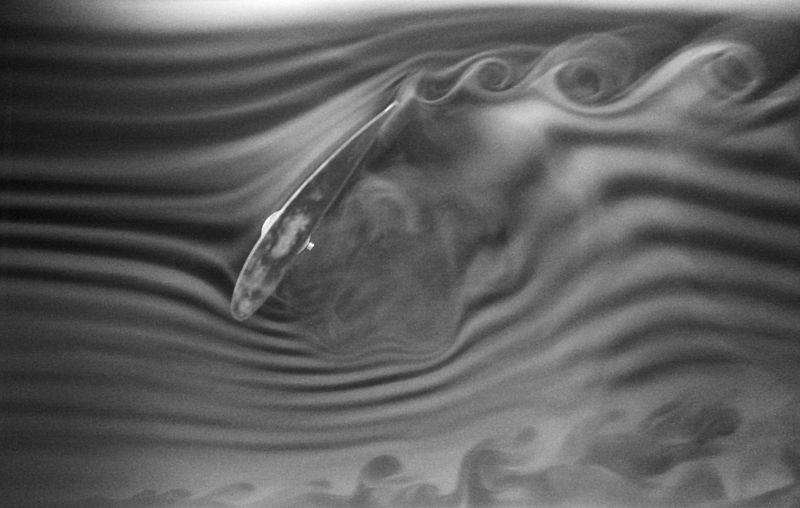
\includegraphics[width=0.6\textwidth]{ImgWindTunnel.jpg}
%  \end{center}
%  \vspace{-20pt}
%  \caption{\small{An airfoil in a fog wind tunnel (image from Wikimedia Commons, Smart Blade GmbH).}}
%\end{figure}
% ~~~~~~~~~~~~~~~~~~~~~~~~~~~~~~~~~~~~~~~~~~~~~~~~~~~~~~~~~
% PARTICLE MOTION
\item 
\textbf{Integration with Vector-Valued Functions}\\
If the position of a particle is given by the vector function $\MB{r}(t) \in \R^3$, then we know that we can determine its velocity, $\MB{v}(t)= \MB{r}'(t)$, by differentiating each of its components. That is, if 
\begin{align*}
  \MB{r}(t) = \BM r_1(t) \\ r_2(t) \\ r_3(t) \EM,
\end{align*}
then
\begin{align*}
  \MB{v}(t)= \MB{r}'(t) = \BM \frac{d}{dt} r_1(t) \\ \frac{d}{dt} r_2(t) \\ \frac{d}{dt} r_3(t) \EM = \BM v_1(t) \\ v_2(t) \\ v_3(t) \EM,
\end{align*}
provided that the derivatives of the components of $\MB{r}$ exist at $t$. It follows from the Fundamental Theorem of Calculus that if we were instead given the velocity of the particle, we could compute its position by integrating each of the components with respect to $t$. We would of course introduce constants of integration. That is, given
\begin{align*}
  \MB{v}(t) = \BM v_1(t) \\ v_2(t) \\ v_3(t) \EM, 
\end{align*}
we could obtain $\MB{r}$ by integrating each of the components of $\MB{v}(t)$
\begin{align*}
  \MB{r}(t) = \BM \int v_1(t) dt \\ \int v_2(t) dt \\ \int v_3(t) dt \EM = \BM r_1(t) + c_1 \\ r_2(t) +c_2 \\ r_3(t) +c_3 \EM,
\end{align*}
where $c_1,c_2,c_3$ are constants. 

Suppose that a particle with mass $m$ is subjected to a force, $\MB{F}(t) = m\pi^2\big(\cos(\pi t)\MB{j}+\sin(\pi t)\MB{k}\big)$, where $t \ge 0$. Suppose also that when $t=0$, 
\begin{align*}
  \MB{r}(0) &= \BM -1 \\ 0 \\ 0 \EM , \quad
  \MB{r}'(0) = \BM +1 \\ 0 \\ 0 \EM.
\end{align*}
\BEN
\item Using the relation $\MB{F} = m\MB{a}$, find the velocity of the particle at time $t$. \textit{Hint: you will need to apply the velocity at time t=0}.
\item Find the position of the particle at time $t=1$.
\item Plot the position of the particle at times $t=0$ and $t=1$ on the same graph in $\R^3$.
\EEN
% ~~~~~~~~~~~~~~~~~~~~~~~~~~~~~~~~~~~~~~~~~~~~~~~~~~~~~~~~~
\EEN % END OF QUESTIONS

